% Imports
\documentclass[9pt, dvipsnames]{beamer}
\usepackage{times}
\usepackage{amsmath}
\usepackage{amsthm}
\usepackage{verbatim}
\usepackage{anyfontsize}
\usepackage{subcaption}
\usepackage{graphicx}
\usepackage[export]{adjustbox}
\usepackage[multidot]{grffile}
\usepackage{tabularx}
\usepackage{tikz}
\usepackage{wasysym}
\usepackage{amsmath,amssymb,amsfonts}
\usepackage{hyperref}

% Beamer Themes
\usetheme{Ilmenau}
\usecolortheme{beaver}
\usefonttheme{professionalfonts}
\setbeamertemplate{caption}[numbered]

% Counter
\newcounter{saveenumi}
\resetcounteronoverlays{saveenumi}

% Preamble
\title{Free and Open Source Software}
\author{James C. Craven}
\date{April 17, 2025}


\begin{document}

\maketitle

%%%%%%%%%%%%%%%%%%%%%%%%%%%%%%%%%%%%%%%%
\section{Introduction}
\begin{frame}{Table of Contents}
    \tableofcontents
\end{frame}

\begin{frame}{Why This Matters}
    \begin{enumerate}
        \pause
        \item Portfolio building
            \begin{itemize}
                \item Personal projects
                \item Contributing to open source
            \end{itemize}
        \pause
        \item Using open source in professional settings
            \begin{itemize}
                \item Legality of using others' projects
                in proprietary code
                \item Working in corporate-owned FOSS
            \end{itemize}
        \pause
        \item Understanding your rights
    \end{enumerate}
\end{frame}

\begin{frame}{Definitions}
    \only<1> {
        \textbf{Free and Open Source Software (FOSS):} \\ Software where the
        source code is made publicly available, allowing anyone to freely use,
        study, modify, and distribute the software.
        \begin{center}
            \begin{figure}
                \centering
                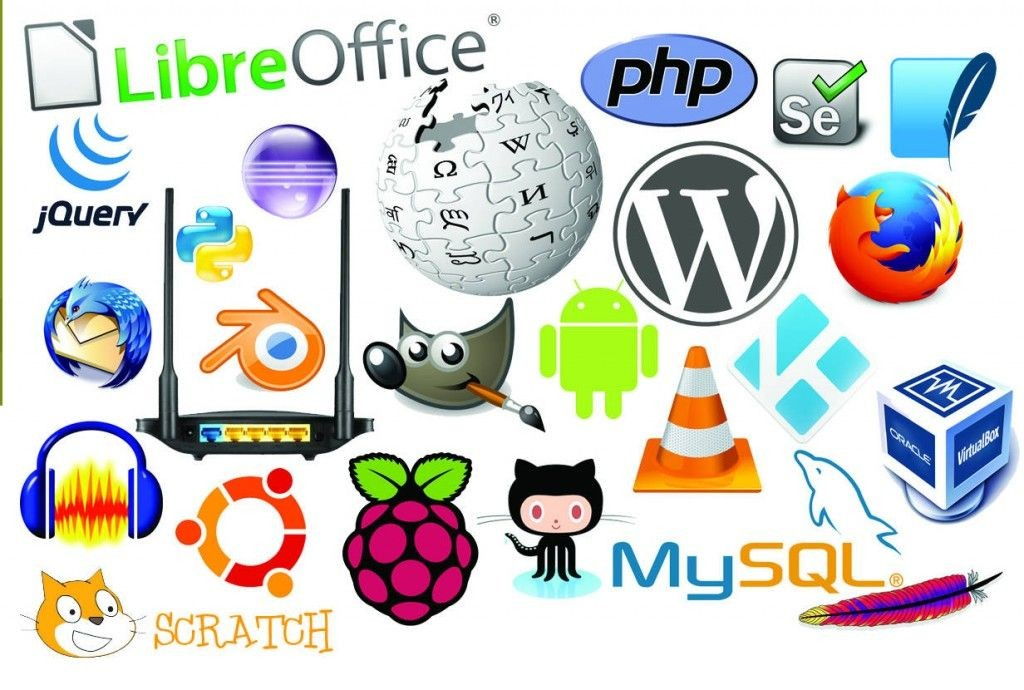
\includegraphics[width=0.7\linewidth]{assets/foss.jpeg}
            \end{figure}
        \end{center}
    }
    \only<2-> {
        \begin{columns}[t]
            \begin{column}{0.5\textwidth}
                \begin{figure}
                    \centering
                    
\includegraphics[height=0.2\paperheight]{assets/GNU.png}
                \end{figure}
                \textbf{Free Software}
                \begin{itemize}
                    \item Four Core Freedoms:
                        \begin{enumerate}
                            \item Use/run program for any purpose
                            \item Study and modify source code
                            \item Redistribute original source code
                            \item Redistribute modified source code
                        \end{enumerate}
                    \item Mostly Ideological: \\ \textit{"Free as in freedom of
                    speech, not free as in beer"}
                \end{itemize}
            \end{column}
            \onslide<3> {
                \begin{column}{0.5\textwidth}
                    \begin{figure}
                        \centering
                        
\includegraphics[height=0.2\paperheight]{assets/OSI.png}
                    \end{figure}
                    \textbf{Open Source}
                    \begin{itemize}
                        \item Rebranding of Free Software Movement to be more
                        appealing
                        \item Focuses on marketing utility of FOSS
                    \end{itemize}
                \end{column}
            }
        \end{columns}
    }
\end{frame}

%%%%%%%%%%%%%%%%%%%%%%%%%%%%%%%%%%%%%%%%
\section{History}

\begin{frame}{The Early Days and Unix}
    \begin{columns}
        \begin{column}{0.5\textwidth}
            \begin{itemize}
                \item In the early 70s, Commercial software was distributed as source
                code.
                \item Users frequently modified and/or distributed modifications to
                software, and it was legal to do so.
                \item By the late 70s, UNIX had thousands of users.
                \item With the rise of general purpose operating systems, desire to
                monetise software increased in the mid 1980s.
            \end{itemize}
        \end{column}
        \begin{column}{0.5\textwidth}
            \begin{figure}
                \centering
                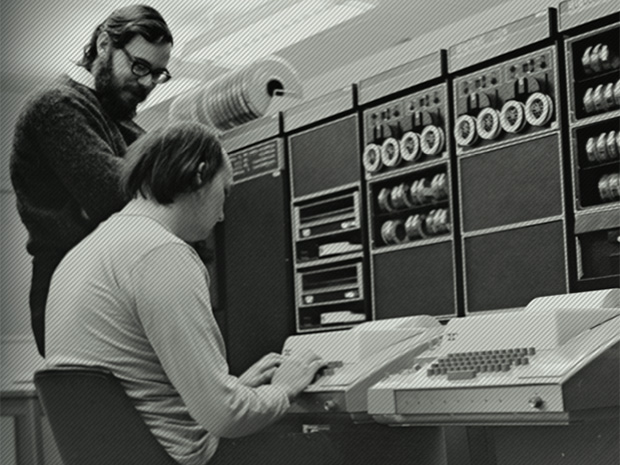
\includegraphics[width=0.8\linewidth]{assets/unix.jpg}
                \caption{Ken Thompson (seated) and Dennis Ritchie in Bell Labs,
                1972}
            \end{figure}
        \end{column}
    \end{columns}
\end{frame}

\begin{frame}{Free Software Movement}
    \begin{columns}
        \begin{column}{0.5\textwidth}
            \begin{itemize}
                \item AT\&T started commercialising UNIX more, and required NDAs
                to receive the software's source code.
                \item Outraged with this, Richard Stallman started the GNU
                project, which intended to build a UNIX-like operating system
                "for free, forever."
                \item Stallman conceived the Four Core Freedoms, and founded the
                Free Software Foundation. His ideas became very influential for
                the next decade to come.
            \end{itemize}
        \end{column}
        \begin{column}{0.5\textwidth}
            \begin{figure}
                \centering
                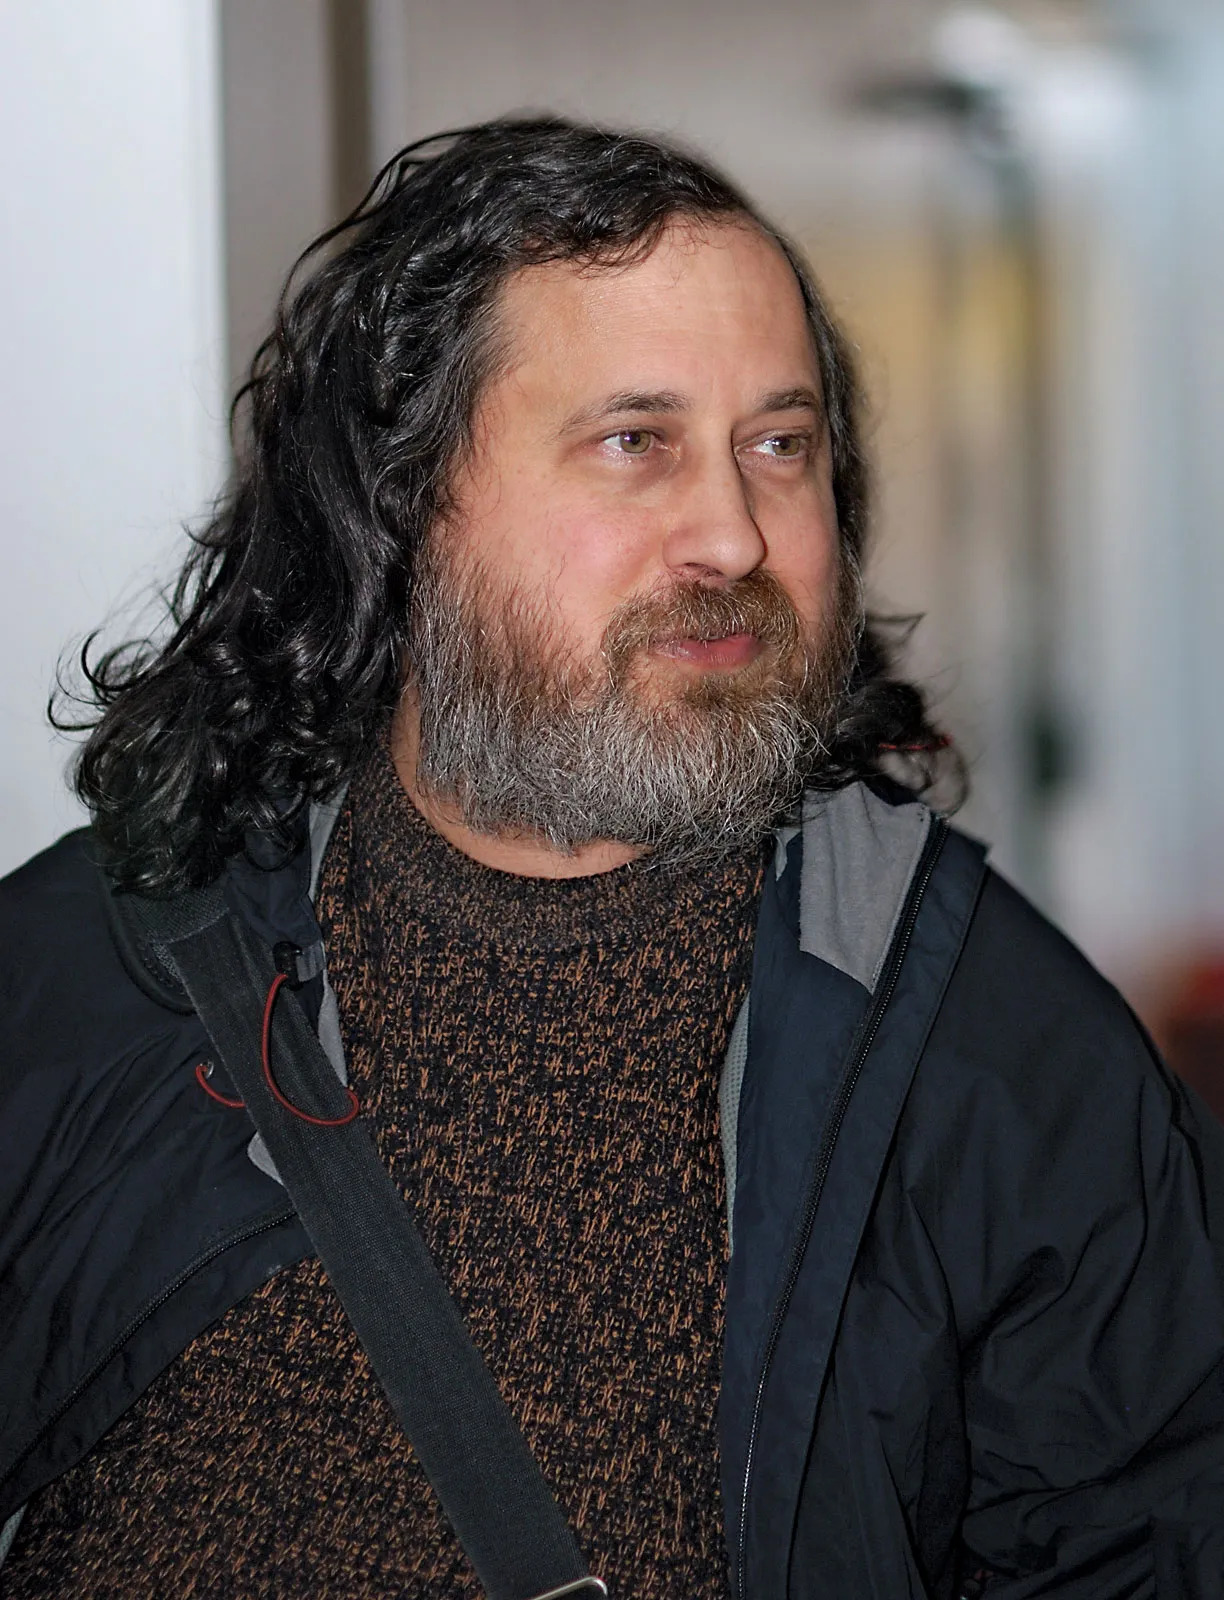
\includegraphics[width=0.6\linewidth]{assets/stallman.jpg}
                \caption{Richard Stallman, founder of the GNU Project.}
            \end{figure}
        \end{column}
    \end{columns}
\end{frame}

\begin{frame}{Open Source Initiative}
    \begin{columns}
        \begin{column}{0.5\textwidth}
            \begin{itemize}
                \item By the early 1990s, the GNU Utilities were complete, but
                the operating system was missing the kernel.
                \item Linus Torvalds, began writing the Linux Kernel, causing
                another surge in interest in free software.
                \item Despite public interest, corporations were hesitant to
                interact with something "free," and thus not monetisable.
                \item In 1998, free software was rebranded as open source
                software. 
            \end{itemize}
        \end{column}
        \begin{column}{0.5\textwidth}
            \begin{figure}
                \centering
                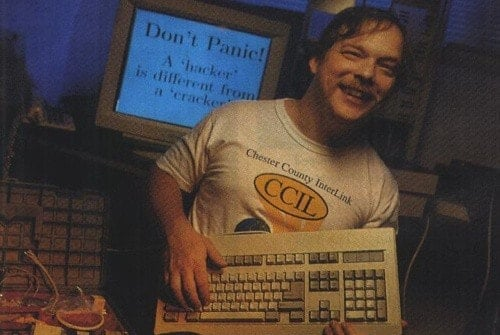
\includegraphics[width=0.7\linewidth]{assets/raymond.jpg}
                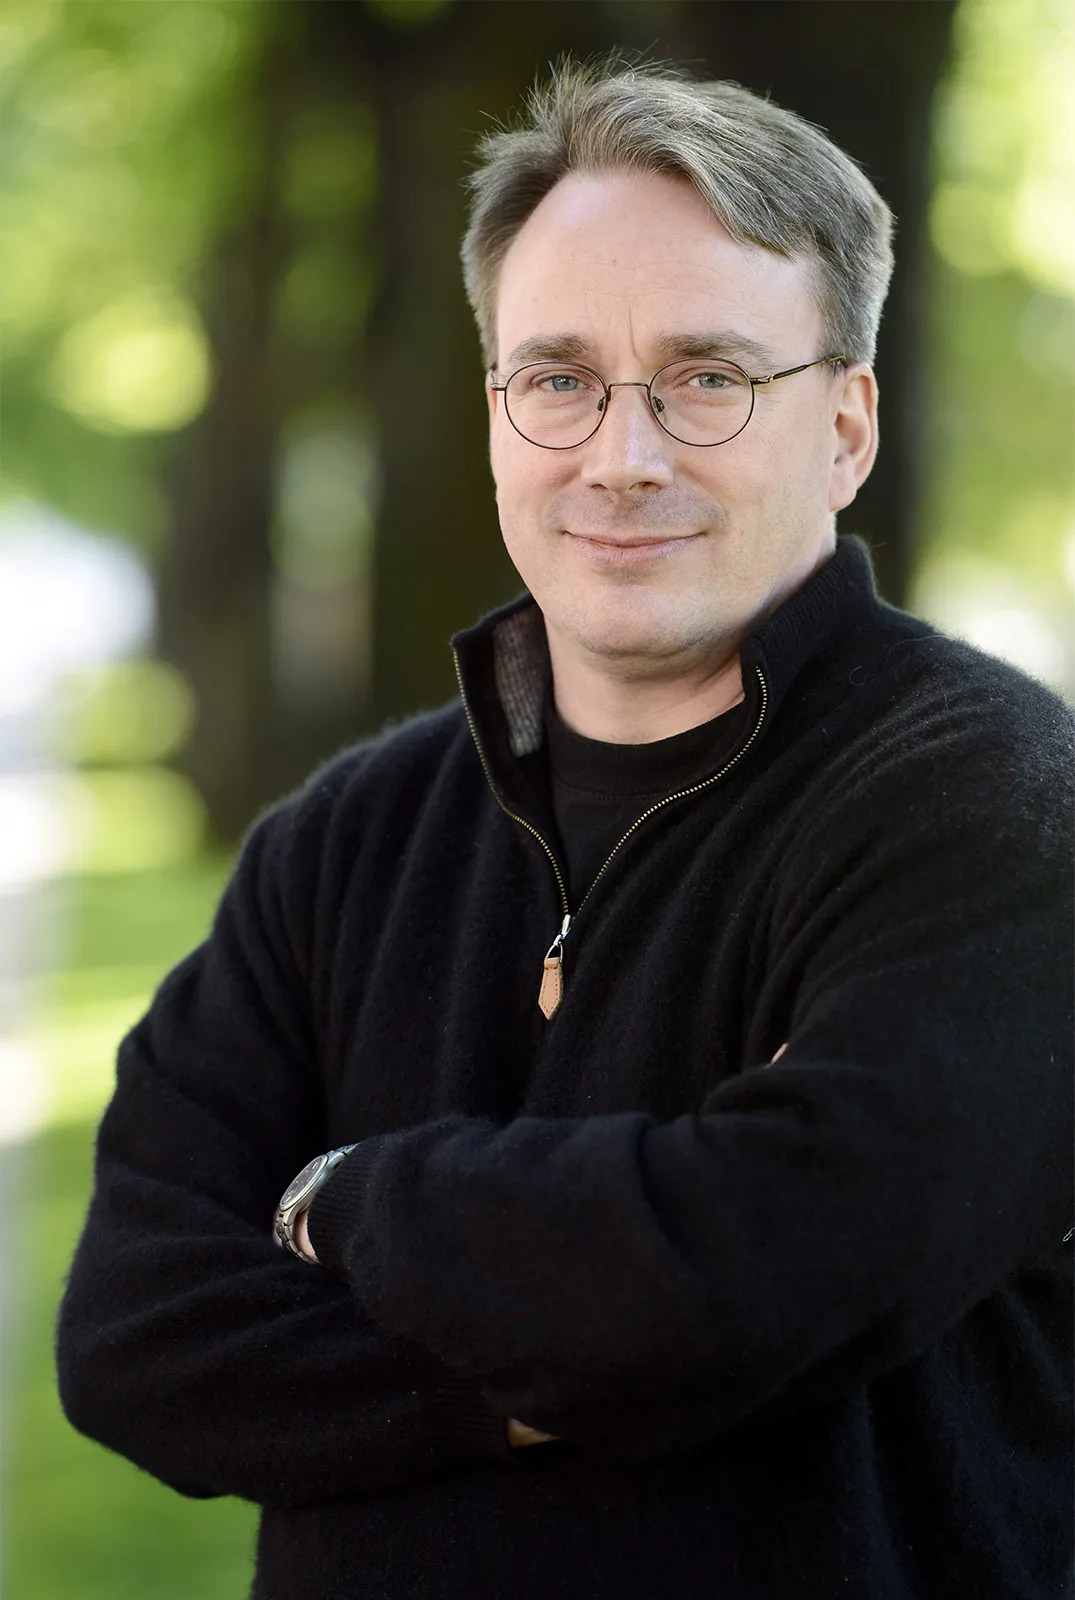
\includegraphics[width=0.3\linewidth]{assets/torvalds.jpg}
                \caption{Eric Raymond, founder of OSI (above) and Linus
                Torvalds, designer of the Linux Kernel (below)}
            \end{figure}
        \end{column}
    \end{columns}
\end{frame}

%%%%%%%%%%%%%%%%%%%%%%%%%%%%%%%%%%%%%%%%
\section{Licenses}

\begin{frame}{Permissive Vs Copyleft}
    The ideological divide gave rise to similar but significantly different
    classes of FOSS licenses: \textbf{Permissive} and \textbf{Copyleft}
    licenses.

    \bigskip

    \begin{center}
        \large
        \begin{tabular}{|l|c|c|}
            \hline
            \textbf{Purpose}  & \textbf{Permissive}  & \textbf{Copyleft} \\
            \hline
            Movement          & OSI        & FSF        \\
            \hline
            Use (Priv./Comm.) & \checkmark & \checkmark \\
            Modify            & \checkmark & \checkmark \\
            Distribute        & \checkmark & \checkmark \\
            Different License & \checkmark & \texttimes \\
            \hline
            Liability         & \texttimes & \texttimes \\
            Warranty          & \texttimes & \texttimes \\
            \hline
        \end{tabular}
    \end{center}
\end{frame}

\begin{frame}{Popular Licenses}
    \begin{itemize}
        \pause
        \item \textbf{GNU Public License (GPL v3):} \\
        Well-known copyleft license created by Stallman and the GNU License.
        \pause
        \item \textbf{MIT License:} \\
        Most popular permissive license. Essentially allows end-user to do
        anything.
        \pause
        \item \textbf{BSD License:} \\
        Permissive license originally created to accompany Berkley Software
        Distribution's fork of UNIX. Exists in 2, 3, and 4 clause forms with
        varying levels of strictness
        \pause
        \item \textbf{Apache License:} \\
        Open Source License created by the Apache Software Foundation. Unique in
        its explicit denial of trademark rights to the product. Affords
        additional protections of GPL without being copyleft
    \end{itemize}
\end{frame}

\begin{frame}{Licenses Summary}
    \begin{center}
        \begin{tabular}{|l|r|c|c|c|c|}
            \hline
            License & Popularity & Copyleft   & Disclose Mod. & Patent     \\
            \hline
            MIT     & 1          & \texttimes & \texttimes    & \texttimes \\
            Apache  & 2          & \texttimes & \checkmark    & \checkmark \\
            GPLv3   & 3          & \checkmark & \checkmark    & \checkmark \\
            BSD 3   & 4-5        & \texttimes & \texttimes    & \texttimes \\
            BSD 2   & 10-12      & \texttimes & \texttimes    & \texttimes \\
            \hline
        \end{tabular}
        {\small \href{https://innovationgraph.github.com/global-metrics/licenses}{https://innovationgraph.github.com/global-metrics/licenses}}
    \end{center}
\end{frame}

\begin{frame}{How to Use Licenses}
    Manually:
    \begin{enumerate}
        \item Create a file in root directory of your project called LICENSE.
        \item Copy and paste the contents of a suitable license into the file.
    \end{enumerate}
    \textbf{OR}, using GitHub:
    \begin{enumerate}
        \item Select add file in your repository
        \item Name the file LICENSE, and select the prompt for a License
        template when prompted
        \item Find a suitable license, and select "review and submit."
        \item Commit the changes when prompted.
    \end{enumerate}
\end{frame}

\section{Conclusion}
\begin{frame}{Conclusion}
    \begin{itemize}
        \item Understanding the software licensing is essential not only for
        your personal projects, but also any other project you contribute to
        publicly or privately.
        \item Copyleft and permissive licenses are similar, but have unique
        aspects that must be considered before usage, especially as a component
        of a larger project.
        \item Licensing your projects is not only important, but it's really
        easy to do and can potentially save you future headaches.
    \end{itemize}
\end{frame}

\begin{frame}{Questions}
    \begin{center}
        {\huge Thank You! Questions?}
        \begin{center}
            
\includegraphics[width=0.4\linewidth]{assets/frame.png}
        \end{center}
    \end{center}
\end{frame}

\end{document}